\documentclass[10pt,french]{article}
%%%%%%%%%%%%%%%%%%%%%%%%%%%%%%%%%%%%%%%%%%%%%%%%%%%%%%%%%%%%%%%%%%%%%%%%%%%%%%%
%___________________________
%===    Configurations 12.09.2013
%------------------------------------------------------
%packages permettant d'augmenter le nombre de registres de dimension et donc d'éviter les erreurs de compilation dûs aux packages tikz, pstricks and compagnie
\usepackage{etex}
%___________________________
%===    Pour le français
%------------------------------------------------------
\usepackage[utf8x]{inputenc}
\usepackage[T1]{fontenc}
\usepackage{babel}
\FrenchFootnotes

%___________________________
%===    Polices d'écriture
%------------------------------------------------------
%\usepackage{mathpazo}
\usepackage{frcursive} % Pour l'écriture cursive
\usepackage[upright]{fourier}% l'option permet d'avoir les majuscules droites dans les formules mathématiques
\usepackage[scaled=0.875]{helvet}

%___________________________
%===    Les couleurs
%------------------------------------------------------
\usepackage[dvipsnames,table]{xcolor}
%
\newcommand{\rouge}[1]{{\color{red} #1}}
\definecolor{midblue}{rgb}{0.145,0.490,0.882}
\newcommand\MaCouleur{midblue}

%___________________________
%===   Redéfinition des marges par défaut
%------------------------------------------------------
\setlength\paperheight{297mm}
\setlength\paperwidth{210mm}
\setlength{\evensidemargin}{0cm}% Marge gauche sur pages paires
\setlength{\oddsidemargin}{0cm}%{-0.5cm}% Marge gauche sur pages impaires
\setlength{\topmargin}{-2cm}% Marge en haut
\setlength{\headsep}{0.5cm}% Entre le haut de page et le texte
\setlength{\headheight}{0.7cm}% Haut de page
\setlength{\textheight}{25.2cm}% Hauteur de la zone de texte
\setlength{\textwidth}{17cm}% Largeur de la zone de texte

\usepackage{lscape} %permet le format paysage du document
\usepackage{xspace} % création automatique d'espaces dans les commandes
\setlength{\parindent}{0pt}

\usepackage{fancyhdr}
\pagestyle{fancy}
%
\renewcommand{\headrulewidth}{0pt}% pas de trait en entête
\newcommand\RegleEntete[1][0.4pt]{\renewcommand{\headrulewidth}{#1}}%commande pour ajouter un trait horizontal en entête

\newcommand{\entete}[3]{\lhead{#1} \chead{#2} \rhead{#3}}
\newcommand{\pieddepage}[3]{\lfoot{#1} \cfoot{#2} \rfoot{#3}}
%
%\renewcommand{\chaptermark}[1]{\markboth{#1}{}} % enregistre le titre courant du chapitre
    %en-tete droite page [paire] et {impaire}
%\rhead[]{\textbf{\leftmark.}}
    %en-tete gauche page [paire] et {impaire}
%\lhead[\textbf{\chaptername~\thechapter.}]{}


\usepackage{enumerate} %permet la modif de la numérotation et de poursuivre une numérotation en cours avec \begin{enumerate}[resume]
\usepackage{enumitem}
\frenchbsetup{StandardLists=true}%frenchb ne s'occupera pas des listes
\setenumerate[1]{font=\bfseries,label=\arabic*\degres)} % numérotation 1°) 2°) ...
%\setenumerate[2]{font=\itshape,label=(\alph*)} % sous-numérotation (a) (b) ...
\setenumerate[2]{font=\bfseries,label=(\alph*)} % sous-numérotation (a) (b) ...

\usepackage{lastpage} % permet d'afficher le nombre total de pages après DEUX compilations.

%___________________________
%===    Raccourcis classe
%------------------------------------------------------
\newcommand\seconde{2\up{nde}\xspace}
\newcommand\premiere{1\up{ère}\xspace}
\newcommand\terminale{T\up{le}\xspace}
\newcommand\stmg{\bsc{Stmg}}
\newcommand\sti{\bsc{Sti2d}}
\newcommand\bat{BAT 1\xspace}
\newcommand\BAT{BAT 2\xspace}
\newcommand\tesspe{TES Spécialité\xspace}


%___________________________
%===    Réglages et Commandes Maths
%------------------------------------------------------
%redéfinition de fractions, limites, sommes, intégrales, coefficients binomiaux en displaystyle, limites de suites
\usepackage{amssymb,mathtools}
\let\binomOld\binom
\renewcommand{\binom}{\displaystyle\binomOld}
\let\limOld\lim
\renewcommand{\lim}{\displaystyle\limOld}
\newcommand{\limn}{\lim_{n\to +\infty}} %limite lorsque n tend vers + infini
\newcommand{\limm}{\lim_{x\to -\infty}} %limite lorsque x tend vers - infini
\newcommand{\limp}{\lim_{x\to +\infty}} %limite lorsque x tend vers + infini
\newcommand{\limz}{\lim_{x\to 0}} %limite lorsque x tend vers 0
\newcommand{\limzm}{\lim_{\substack{x \to 0\\ x < 0}}} %limite lorsque x tend vers 0-
\newcommand{\limzp}{\lim_{\substack{x \to 0\\ x > 0}}} %limite lorsque x tend vers 0+
\let\sumOld\sum
\renewcommand{\sum}{\displaystyle\sumOld}
\let\intOld\int
\renewcommand{\int}{\displaystyle\intOld}

%\usepackage{yhmath}%permet les arcs de cercles
%\usepackage[euler-digits]{eulervm} %-> police maths
%
\usepackage{amssymb,mathtools}
\usepackage{stmaryrd}%\llbracket et \rrbracket % crochets doubles pour intervalles d'entier
%symbole parallèle avec \sslash

\newcommand{\crochets}[2]{\ensuremath{\llbracket #1 ; #2 \rrbracket}}

\newcommand{\intervalleff}[2]{\left[#1\,;#2\right]}
\newcommand{\intervallefo}[2]{\left[#1\,;#2\right[}
\newcommand{\intervalleof}[2]{\left]#1\,;#2\right]}
\newcommand{\intervalleoo}[2]{\left]#1\,;#2\right[}



\usepackage{bm} % pour l'écriture en gras des formules mathématiques avec \bm

\usepackage{cancel} % pour les simplifications de fractions
\renewcommand\CancelColor{\color{red}}
%\usepackage{siunitx} % écriture de nombres et d'unités
%\sisetup{output-decimal-marker={,},detect-all}
\usepackage[autolanguage,np]{numprint}
%permet les espacement pour les nombres décimaux avec \np{3,12456} en environnement maths ou pas
\DecimalMathComma %supprime l'espace après la virgule dans un nombre

%
\usepackage{dsfont} %écriture des ensemble N, R, C ...
\newcommand{\C}{\mathds C}
\newcommand{\R}{\mathds R}
\newcommand{\Q}{\mathds Q}
\newcommand{\D}{\mathds D}
\newcommand{\Z}{\mathds Z}
\newcommand{\N}{\mathds N}
\newcommand\Ind{\mathds 1} %= fonction indicatrice
\newcommand\p{\mathds P} %= probabilité
\newcommand\E{\mathds E} % Espérance
\newcommand\V{\mathds V} % Variance
\newcommand{\e}{\text{e}}
\newcommand{\dd}{\,\text{d}}

%Nombres complexes
\let\Reold\Re
\renewcommand{\Re}{~\text{Re}~}
\let\Imold\Im
\renewcommand{\Im}{~\text{Im}~}
\newcommand{\ii}{\,\text{i}}
% Exponentielle complexe
\newcommand{\ei}[2]{\,\e^{\dfrac{#1\ii\pi}{#2}}}


%
\usepackage{mathrsfs}   % Police de maths jolie caligraphie
\newcommand{\calig}[1]{\ensuremath{\mathscr{#1}}}
\newcommand\mtc[1]{\ensuremath{\mathcal{#1}}}


%Gestion des espaces
%
\newcommand{\pv}{\ensuremath{\: ; \,}}
\newlength{\EspacePV}
\setlength{\EspacePV}{1em plus 0.5em minus 0.5em}
\newcommand{\qq}{\hspace{\EspacePV} ; \hspace{\EspacePV}}
\newcommand{\qetq}{\hspace{\EspacePV} \text{et} \hspace{\EspacePV}}
\newcommand{\qouq}{\hspace{\EspacePV} \text{ou} \hspace{\EspacePV}}
\newcommand{\qLq}{\hspace{\EspacePV} \Leftarrow \hspace{\EspacePV}}
\newcommand{\qRq}{\hspace{\EspacePV} \Rightarrow \hspace{\EspacePV}}
\newcommand{\qLRq}{\hspace{\EspacePV} \Leftrightarrow \hspace{\EspacePV}}

%simplification notation norme \norme{}
\newcommand{\norme}[1]{\left\Vert #1\right\Vert}


%simplification de la notation de vecteur \vect{}
\newcommand{\vect}[1]{\mathchoice%
{\overrightarrow{\displaystyle\mathstrut#1\,\,}}%
{\overrightarrow{\textstyle\mathstrut#1\,\,}}%
{\overrightarrow{\scriptstyle\mathstrut#1\,\,}}%
{\overrightarrow{\scriptscriptstyle\mathstrut#1\,\,}}}



%Repères
\def\Oij{$\left(\text{O}\pv\vect{\imath},~\vect{\jmath}\right)$\xspace}
\def\Oijk{$\left(\text{O}\pv\vect{\imath},~ \vect{\jmath},~ \vect{k}\right)$\xspace}
\def\Ouv{$\left(\text{O}\pv\vect{u},~\vect{v}\right)$\xspace}
\def\OIJ{$\left(O\pv I\:,\,J\right)$\xspace}

\newcommand\abs[1]{\ensuremath{\left\vert #1 \right\vert}}%valeur absolue
\newcommand\Arc[1]{\ensuremath{\wideparen{#1}}}%arc de cercle


%symbole pour variable aléatoire qui suit une loi
\newcommand{\suit}{\hookrightarrow}

%___________________________
%===    Pour les tableaux
%------------------------------------------------------
\usepackage{array}
\usepackage{longtable}
\usepackage{tabularx,tabulary}
\usepackage{multirow}
\usepackage{multicol}
%exemple
%\begin{multicols}{3}[Titre sur une seule colonne.]
%   3~colonnes équilibrées, 3~colonnes équilibrées, 3~colonnes équilibrées, 3~colonnes équilibrées
%\end{multicols}
%\begin{multicols}{2}[\section{Titre numéroté.}]
%   blabla sur deux colonnes, c'est plus sérieux. C'est le style qui est généralement utilisé pour écrire des articles.
%saut de colonne forcé :
%\columnbreak
%djhskjdhjsq
%sdkksqjhd
%\end{multicols}
%Pour ajouter un titre numéroté qui apparaisse sur toute la largeur de la page, il faut utiliser l'option [\section{Titre.}] juste après \begin{multicols}{nb-col}.
%Remarques :
%Pour qu'une ligne de séparation apparaisse entre les colonnes, il faut utiliser : \setlength{\columnseprule}{1pt}.

%Pour redéfinir la largeur de l'espace inter-colonnes, il faut utiliser \setlength{\columnsep}{30pt}.

%Pour remonter le texte, dans chaque colonne vers le haut : \raggedcolumns qui se tape :\begin{multicols}{2}\raggedcolumns...\columnbreak...\columnbreak\end{multicols}

%Pour supprimer les traits verticaux : \setlength{\columnseprule}{0pt} avant \begin{multicols}{3}...\end{multicols}
\setlength\columnseprule{0.4pt}
\renewcommand{\arraystretch}{1.5}%augmente la hauteur des lignes des tableaux
%colonnes centrées verticalement et horizontalement permettant d'écrire des paragraphes de largeur fixée du type M{3cm}
\newcolumntype{M}[1]{>{\centering\arraybackslash}m{#1}}%cellule centrée horizontalement et verticalement
%\arraybackslash permet de continuer à utiliser \\ pour le changement de ligne

\usepackage{arydshln}% permet des filets horizontaux ou verticaux en pointillés avec
%pour les filets horizontaux \hdashline ou \cdashline qui s'utilisent comme \hline ou \cline
% pour les filets verticaux les deux points :


%___________________________
%===    Divers packages
%------------------------------------------------------
\usepackage{bclogo}
\usepackage{textcomp}
\usepackage{eurosym}%avec \EUR{3,12}
\usepackage{soul} % Pour souligner : \ul
\usepackage{ulem} % Pour souligner double : \uuline
                      % Pour souligner ondulé : \uwave
                      % Pour barrer horizontal : \sout
                      % Pour barrer diagonal : \xout
\usepackage{tikz,tkz-tab,tkz-graph}
\usetikzlibrary{calc,shapes,arrows,plotmarks,lindenmayersystems,decorations,decorations.pathreplacing,patterns}
\usepackage{pstricks,pst-plot,pst-text,pstricks-add,pst-eucl,pst-all}


%INTERLIGNES
\usepackage{setspace}
%s'utilise avec \begin{spacing}{''facteur''}
%   […]
%\end{spacing}

%Pointillés sur toute la ligne
\usepackage{multido}
\newcommand{\Pointilles}[1][1]{%
\multido{}{#1}{\makebox[\textwidth]{\dotfill}\\[1.5\parskip]
}}
%commandes : \Pointilles ou \Pointilles[4] pour 4 lignes


%textes à trous
\newlength\lgtrou
\newcommand*\trou[1]{%
\settowidth\lgtrou{#1}%
\makebox[2\lgtrou]{\dotfill}
\setlength\baselineskip{1.2\baselineskip}}
%Commande à utiliser : \trou{texte qui sera remplacé par des pointillés}

%divers cadres
\usepackage{fancybox} % par exemple \ovalbox{}

%caractères spéciaux avec la commande \ding{230} par exemple
\usepackage{pifont}

%___________________________
%===    Quelques raccourcis perso
%------------------------------------------------------
\newcommand\pfr[1]{\psframebox[linecolor=red]{#1}}
\newcommand\coef[1][]{c{\oe}fficient#1\xspace}


%QRcode, codebarre
\usepackage{pst-barcode}
%\begin{pspicture}(2,2)
%	\psbarcode{http://www.latex-howto.be}{eclevel=M}{qrcode}
%\end{pspicture}


%Texte en filigrane
\usepackage{watermark}
%On utilise ensuite les commandes \watermark, \leftwatermark, \rightwatermark ou \thiswatermark qui permettent de définir un filigrane sur toutes les pages, les pages paires, les pages impaires ou juste une page
%Exemple : \thiswatermark {
%\begin{minipage}{0.95\linewidth}
%\vspace{25cm}
%\begin{center}
%\rotatebox{55}{\scalebox{8}{\color[gray]{0.7}\LaTeX}}
%\end{center}
%\end{minipage}
%}

%QCM
\usepackage{alterqcm}					%%Permet de créer des QCM
%\begin{alterqcm}
%\AQquestion{Question}{{Proposition 1},{Proposition 2},{Proposition 3}}
%\end{alterqcm}

%\dingsquare %carré avant V ou F
%\dingchecksquare %carré validé devant V ou F


%Rond entourant une lettre avec pour arguments la couleur de fond, puis la lettre
\newcommand\rond[2][red!20]{\tikz[baseline]{\node[fill=#1,anchor=base,circle]{\bf #2};}}


%Ecrire card en écriture normale :
\newcommand{\card}{\text{card}\xspace}


%___________________________
%===    ALGORITHMES
%------------------------------------------------------

%ALGORITHME avec Algobox
\usepackage{ucs}
\usepackage{framed}
\definecolor{fond}{gray}{0.95}
\newenvironment{cadrecode}{%
  \def\FrameCommand{{\color[HTML]{888888}\vrule width 3pt}\colorbox{fond}}%
  \MakeFramed {\advance\hsize-\width \FrameRestore}}%
{\endMakeFramed}
\usepackage{alltt}

% Mise en forme des algorithmes
\usepackage[french,boxed,titlenumbered,lined,longend]{algorithm2e}
  \SetKwIF {Si}{SinonSi}{Sinon}{si}{alors}{sinon\_si}{alors}{fin~si}
 \SetKwFor{Tq}{tant\_que~}{~faire~}{fin~tant\_que}
 \SetKwFor{PourCh}{pour\_chaque }{ faire }{fin pour\_chaque}
 \SetKwInput{Sortie}{Sortie}
  \SetKwInput{Entree}{Entrée}
\newcommand{\Algocmd}[1]{\textsf{\textsc{\textbf{#1}}}}\SetKwSty{Algocmd}
  \newcommand{\AlgCommentaire}[1]{\textsl{\small  #1}}


%___________________________
%===    MISE EN FORME EXERCICES
%------------------------------------------------------
%\usepackage{marvosym}
\usepackage{slashbox}

\newcounter{exo}
\newenvironment{exo}{%
  \refstepcounter{exo}\Writinghand\ \textbf{Exercice \theexo.}\par
  \medskip}%
{\[*\]}


%___________________________
%===    HYPERLIENS
%------------------------------------------------------
\usepackage[colorlinks=true,linkcolor=black,filecolor=blue,urlcolor=blue,bookmarksnumbered]{hyperref} 

\newcounter{exercice}\newcommand{\exercice}{\refstepcounter{exercice}\textbf{\large{Exercice \theexercice \ :}}\xspace}

\fancypagestyle{garde_tete}{
    \fancyhead[C]{
        \small\textbf{\seconde} \hfill \small \textbf{Année 2013-2014}
                           }
    \renewcommand{\headrulewidth}{0cm}
}

\newcommand{\tete}{
    \thispagestyle{garde_tete}
        
\begin{tikzpicture}
            \node[shading=ball,ball color=blue!20,rectangle,draw=black,rounded corners,thick]{%
                \begin{minipage}{\linewidth}
                    \begin{center}
                        \vspace*{9pt}
                            \Large \textsc{\textbf{Correction du devoir commun de mathématiques}}
                        \vspace*{9pt}
                    \end{center}
                \end{minipage}
            };
        \end{tikzpicture}
\noindent
\vspace{-6pt}
}



%-------------------------------------------------------------------------
%        DEBUT DU DOCUMENT
%-------------------------------------------------------------------------


\begin{document}

\setlength\parindent{0mm}
\tete 		%entête classique

\renewcommand \footrulewidth{0.2pt}%
\renewcommand \headrulewidth{0pt}%
\pagestyle{fancy}
\fancyhf{}
\pieddepage{\seconde}{\thepage / \pageref{LastPage}}{Année 2013-2014}



%-------------------------------------------------------------------------
%        EXERCICE 1
%-------------------------------------------------------------------------


\exercice \hfill\textbf{(15 points)}%inspiré de l'ex 80 p 191 Hyperbole
\bigskip

La figure complétée est la suivante :

\begin{center}
    \begin{tikzpicture}[scale=0.7,line cap=round,line join=round,>=stealth,x=1.0cm,y=1.0cm]
    \clip(-9.5,-11.5) rectangle (8.5,8.5);%%%%%%%%%%%%réduit la fenêtre d'affichage de ce qui suit

        %grille
        \draw [color=gray!50, xstep=0.5,ystep=0.5] (-9.5,-11.5) grid (8.5,8.5);
        \draw [color=gray,xstep=1.0,ystep=1.0] (-9.5,-11.5) grid (8.5,8.5);

        %droites

        \draw[smooth,samples=200,domain=-9.5:8.5,line width=1.5pt] plot(\x,{5*\x+1});
        \draw (-3,-11) node [above right,font=\bfseries] {\calig{D}};
        \draw[smooth,samples=200,domain=-9.5:8.5,line width=1.5pt,color=OliveGreen,style=dashed] plot(\x,{2*\x+4});
        \draw[smooth,samples=200,domain=-9.5:8.5,line width=1.5pt,color=red] plot(\x,{-(\x)+1});
        \draw (-4,5) node [above right,font=\boldmath] {$\Delta$};
        \draw[smooth,samples=200,domain=-9.5:8.5,line width=1.5pt,color=red] plot(\x,{-(\x)-11});



        %axes
        \draw[->,line width=2pt] (-9.5,0) -- (8.5,0);
        \foreach \times in {-9,...,8}
        \draw[color=black] (\times,2pt) -- (\times,-2pt) node[below,font=\boldmath] {$\times$};
        \draw[->,line width=2pt] (0,-11.5) -- (0,8.5);
        \foreach \y in {-11,...,8}
        \draw[color=black] (2pt,\y) -- (-2pt,\y) node[left,font=\boldmath] {$\y$};

        %triangle
        \draw [line width=1.5pt,color=blue] (-2,3)--(-2,-9)--(-8,-3)--cycle;

        %points
        \draw (-2,3) node [above right,font=\bfseries] {A};
        \draw [line width=1.5pt] (-2,3)-- ++(3pt,3pt)-- ++(-6pt,-6pt)-- ++(3pt,3pt)-- ++(-3pt,3pt)-- ++(6pt,-6pt);
        \draw (0,1) node [above right,font=\bfseries] {B};
        \draw [line width=1.5pt] (0,1)-- ++(3pt,3pt)-- ++(-6pt,-6pt)-- ++(3pt,3pt)-- ++(-3pt,3pt)-- ++(6pt,-6pt);
        \draw (-2,-9) node [below left,font=\bfseries] {C};
        \draw [line width=1.5pt] (-2,-9)-- ++(3pt,3pt)-- ++(-6pt,-6pt)-- ++(3pt,3pt)-- ++(-3pt,3pt)-- ++(6pt,-6pt);
        \draw (-8,-3) node [below left,font=\bfseries] {D};
        \draw [line width=1.5pt] (-8,-3)-- ++(3pt,3pt)-- ++(-6pt,-6pt)-- ++(3pt,3pt)-- ++(-3pt,3pt)-- ++(6pt,-6pt);
        \draw (-1,2) node [below left,font=\bfseries] {I};
        \draw [line width=1.5pt] (-1,2)-- ++(3pt,3pt)-- ++(-6pt,-6pt)-- ++(3pt,3pt)-- ++(-3pt,3pt)-- ++(6pt,-6pt);
        \draw (-5,-6) node [below left,font=\bfseries] {K};
        \draw [line width=1.5pt] (-5,-6)-- ++(3pt,3pt)-- ++(-6pt,-6pt)-- ++(3pt,3pt)-- ++(-3pt,3pt)-- ++(6pt,-6pt);
        \draw (1,6) node [below right,font=\boldmath] {$\Omega$};
        \draw [line width=1.5pt] (1,6)-- ++(3pt,3pt)-- ++(-6pt,-6pt)-- ++(3pt,3pt)-- ++(-3pt,3pt)-- ++(6pt,-6pt);
    \end{tikzpicture}
\end{center}

\begin{enumerate}[label=\arabic*.]
\item 	\begin{enumerate}[label=\alph*)]
	\item %Dans le repère ci-dessus, lire les coordonnées des points A et B.
	Le point A a pour coordonnées $(-2\pv 3)$.

	\item %Placer les points $C(-2\pv -9)$ et $D(-8\pv -3)$.
	Voir la figure.
	
	
	\end{enumerate}

\item %Quelle est la nature du triangle ADC ? Justifier.
	Dans le repère orthonormé précédent, on a :
	
	$AC^2=\left( x_C-x_A\right)^2+\left( y_C-y_A\right)^2=[-2-(-2)]^2+(-9-3)^2=144$,
	
	$AD^2=\left( x_D-x_A\right)^2+\left( y_D-y_A\right)^2=[-8-(-2)]^2+(-3-3)^2=72$, et
	
	$DC^2=\left( x_C-x_D\right)^2+\left( y_C-y_D\right)^2=[-2-(-8)]^2+[-9-(-3)]^2=72$.
	
	Ainsi $AD^2=DC^2$, donc $AD=DC$ et le triangle ADC est isocèle en D.
	
	De plus, $AD^2+DC^2=72+72=144=AC^2$.
	
	D'après la réciproque du théorème de Pythagore, le triangle ADC est rectangle en D.
	
	Le triangle ADC est donc rectangle et isocèle en D.

\item 	\begin{enumerate}[label=\alph*)]
	\item %Déterminer, par le calcul, une équation de la droite $(CD)$.
	$x_C\neq x_D$, donc la droite $(CD)$ admet une équation du type $y=mx+p$.
	
	$m=\dfrac{y_D-y_C}{x_D-x_C}=\dfrac{-3-(-9)}{-8-(-2)}=\dfrac{6}{-6}=-1$.
	
	La droite $(CD)$ admet donc une équation du type $y=-x+p$.
	
	$C\in (CD)$ donc $y_C=-x_C+p$.
	
	Or, $y_C=-x_C+p\qLRq -9=-(-2)+p\qLRq -11=p$.
	
	La droite $(CD)$ admet donc pour équation (réduite) $y=-x-11$.
	
	\item %Déterminer, par le caul, une équation de la droite $\Delta$ parallèle à la droite $(CD)$ passant par $A$.
	La droite $(CD)$ n'est pas parallèle à l'axe des ordonnées.
	
	La droite $\Delta$ ne l'est donc pas non plus et admet le même c\oe{}fficient directeur que la droite $(CD)$.
	
	Elle admet donc une équation du type $y=-x+p'$.
	
	$A\in \Delta\Leftrightarrow y_A=-x_A+p'\Leftrightarrow 3=2+p'\Leftrightarrow 1=p'$.
	
	$\Delta$ admet pour équation $y=-x+1$.
		
	\end{enumerate}

\item 	\begin{enumerate}[label=\alph*)]
	\item \calig{D} a pour équation $y=5x+1$.
	
	$\star$ Pour $x=0$ : $y=5\times 0+1=1$
	
	$\star$ Pour $x=-2$ : $y=5\times (-2)+1=-9$
	
	La droite \calig{D} passe donc par les points de coordonnées $(0\pv 1)$ et $(-2\pv -9)$.
	
	\item Notons $(x\pv y)$ les coordonnées du point B.
	
	Remarquons tout d'abord que B existe car $\calig{D}$ et $\Delta$ sont sécantes : elles n'ont pas le même c\oe{}fficient directeur.
	
	Le couple $(x\pv y)$ est solution du système $(S) : \left\{\begin{array}{rcl}
	y&=&-x+1\\
	y&=&5x+1
	\end{array}\right.
	$.
	
	Or, $(S)\Leftrightarrow \left\{\begin{array}{rcl}
	y&=&-x+1\\
	-x+1&=&5x+1
	\end{array}\right.\Leftrightarrow \left\{\begin{array}{rcl}
	y&=&-x+1\\
	0&=&6x
	\end{array}\right.\Leftrightarrow\left\{\begin{array}{rcl}
	y&=&-0+1\\
	0&=&x
	\end{array}\right.\Leftrightarrow \left\{\begin{array}{rcl}
	y&=&1\\
	x&=&0
	\end{array}\right.$
	
	Les coordonnées du point B sont $(0\pv 1)$.
	
	\textcolor{blue}{Remarquons que les deux droites en question ont la même ordonnée à l'origine : 1. Elles passent donc toutes les deux par le point de coordonnées $(0\pv 1)$. On retrouve le résultat précédent.}
	\end{enumerate}

\item
	\begin{enumerate}[label=\alph*)]
	\item Comme $\Omega\in \calig{D}$, $y_{\Omega}=5x_{\Omega}+1=5\times 1+1=6$.
	
	L'ordonnée de $\Omega$ est de 6.
	
	\item Comme K est le milieu du segment $[CD]$,
	
	$x_K=\dfrac{x_C+x_D}{2}=\dfrac{-2-(-8)}{2}=-5\qetq y_K=\dfrac{y_C+y_D}{2}=\dfrac{-9+(-3)}{2}=-6$.
	
	K a pour coordonnées $(-5\pv -6)$.
	
	\item %Les points $\Omega$, I et K sont-ils alignés ?
	\textbf{1\up{ère} méthode :}
	
	$\star$ $x_{\Omega}\neq x_K$, donc la droite $(K\Omega)$ a pour c\oe{}fficient directeur $m_1=\dfrac{y_\Omega-y_K}{x_{\Omega}-x_K}=\dfrac{6-(-6)}{1-(-5)}=2$.
	
	$\star$ $x_{\Omega}\neq x_I$, donc la droite $(I\Omega)$ a pour c\oe{}fficient directeur $m_2=\dfrac{y_\Omega-y_I}{x_{\Omega}-x_I}=\dfrac{6-2}{1-(-1)}=2$.
	
	$m_1=m_2$, donc les points I, K et $\Omega$ sont alignés.
	
	\textbf{2\up{ème} méthode :}
	
	$\star$ Déterminons une équation de la droite $(IK)$.
	
	$x_I\neq x_K$, donc la droite $(IK)$ admet une équation du type $y=ax+b$.
	
	$a=\dfrac{y_I-y_K}{x_I-x_K}=\dfrac{2-(-6)}{-1-(-5)}=2$.
	
	La droite $(IK)$ admet une équation du type $y=2x+b$.
	
	$I\in (IK)$, donc $y_I=2x_I+b$.
	
	Or, $y_I=2x_I+b\qLRq 2=2\times (-1)+b\qLRq 4=b$.
	
	La droite $(IK)$ admet pour équation $y=2x+4$.
	
	$\star$ Vérifions si le point $\Omega$ appartient ou non à la droite $(IK)$.
	
	$2x_{\Omega}+4=2\times 1+4=6=y_{\Omega}$, donc $\Omega\in (IK)$.
	
	Conclusion : Les points I, K et $\Omega$ sont alignés.
	\end{enumerate}
\end{enumerate}

\begin{center}
$\star$\quad $\star$\quad $\star$\quad $\star$\quad $\star$
\end{center}



%-------------------------------------------------------------------------
%        EXERCICE 2
%-------------------------------------------------------------------------


\exercice \hfill\textbf{(15 points)}%
\bigskip

%--------------------------------------------------------------------------------------
\textbf{Partie} \rond{A}
%---------------------------------------------------------------------------------------


%La courbe représentative $\calig{C}_f$ de la fonction $f$ est tracée dans le repère orthogonal ci-dessous.

\begin{enumerate}[label=\arabic*.]
\item %Lire les images par $f$ des nombres $-6$ ; $-3$ et $8$.
$\star$ L'image de $-6$ par $f$ est $100$.

$\star$ L'image de $-3$ par $f$ est $-150$.

$\star$ L'image de $8$ par $f$ est $0$.

\begin{center}
        \begin{tikzpicture}[scale=0.8,line cap=round,line join=round,>=stealth,x=1cm,y=0.02cm]
            \draw[gray] (-8,-300)grid(8,500);
            \draw[->,line width=1.5pt] (-8,0)--(8,0)node[below,font=\boldmath] {$x$};
            \draw[->,line width=1.5pt] (0,-300)--(0,500)node[left,font=\boldmath] {$y$};
            \foreach \times in {-7,-6,-5,-4,-3,-2,-1,1,2,3,4,5,6,7}
            \draw (\times,2pt) -- (\times,-2pt) node[below,font=\bfseries] {\times};
            \draw (1.5,-25) node[below,font=\bfseries] {1,5};
            \foreach \y in {-250,-200,-150,-100,-50,50,100,150,200,250,300,350,400,450}
            \draw[color=black] (2pt,\y) -- (-2pt,\y) node[left,font=\bfseries] {\y};
            \draw (-2pt,-2pt) node [below left,font=\bfseries] {0};

            \draw[line width=1.5pt] plot[smooth=200,mark=x,mark options={scale =2.5}] coordinates{(-8,400)(-7,200)(-6,100)(-5,0)(-4,-100)(-3,-150)(-2,-100)(-1,0)(0,50)(1.5,100)(3,200)(6,100)(7,50)(8,0)};
            \draw[line width=2pt,style=dashed](1.5,0)--(1.5,100)--(0,100);
            \draw (-7,300) node[above right,font=\boldmath]{$\calig{C}_f$};
            \clip (-8,-300) rectangle (8,500);
            \draw [smooth,samples=200,domain=-8:8,line width=1.5pt,color=red] plot(\x,{2*(\x)^3-3*(\x)^2-72*(\x)+208});
            \draw (7,250) node [above left,font=\boldmath] {$\calig{C}_g$};
        \end{tikzpicture}
    \end{center}



\item %Lire les antécédents de $200$ par la fonction $f$.
Graphiquement $200$ admet deux antécédents par $f$ dans l'intervalle $\intervalleff{-8}{8}$ : $-7$ et $3$.

\item %Résoudre graphiquement, sur l'intervalle $\intervalleff{-8}{8}$, l'inéquation $f(x)\geq 0$.
Graphiquement, l'ensemble des solutions de l'inéquation $f(x)\geq 0$ sur l'intervalle $\intervalleff{-8}{8}$ est $\intervalleff{-8}{-5}\cup\intervalleff{-1}{8}$.

\item 	\begin{enumerate}[label=\alph*)]
	\item On obtient le tableau de variation suivant de $f$ dans l'intervalle $\intervalleff{-8}{8}$ :
	%:-+-+-+-+- Engendré par : http://math.et.info.free.fr/TikZ/TableauxVariations/

\begin{center}
    \begin{tikzpicture}
        \tkzTabInit[espcl=2.5]{$x$/0.75,Variations \\ de $f$/1.5}{$-8$,$-3$,$3$,$8$}
        \tkzTabVar{+/$400$,-/$-150$,+/$200$,-/$0$}
    \end{tikzpicture}
\end{center}
%
%
%\begin{center}
%\begin{tikzpicture}[scale=0.875]
%% Styles
%\tikzstyle{cadre}=[thin]
%\tikzstyle{fleche}=[->,>=latex,thin]
%\tikzstyle{nondefini}=[lightgray]
%% Dimensions Modifiables
%\def\Leftrightarrowg{1.5}
%\def\HtX{1}
%\def\HtY{0.5}
%% Dimensions Calculées
%\def\lignex{-0.5*\HtX}
%\def\lignef{-1.5*\HtX}
%\def\separateur{-0.5*\Leftrightarrowg}
%% Largeur du tableau
%\def\gauche{-1.5*\Leftrightarrowg}
%\def\droite{6.5*\Leftrightarrowg}
%% Hauteur du tableau
%\def\haut{0.5*\HtX}
%\def\bas{-1.5*\HtX-2*\HtY}
%% Ligne de l'abscisse : x
%\node at (-1*\Leftrightarrowg,0) {$x$};
%\node at (0*\Leftrightarrowg,0) {$-8$};
%\node at (2*\Leftrightarrowg,0) {$-3$};
%\node at (4*\Leftrightarrowg,0) {$3$};
%\node at (6*\Leftrightarrowg,0) {$8$};
%% Ligne de la fonction : f(x)
%\node  at (-1*\Leftrightarrowg,{-1*\HtX+(-1)*\HtY}) {$f$};
%\node (f1) at (0*\Leftrightarrowg,{-1*\HtX+(0)*\HtY}) {$400$};
%\node (f2) at (2*\Leftrightarrowg,{-1*\HtX+(-2)*\HtY}) {$-150$};
%\node (f3) at (4*\Leftrightarrowg,{-1*\HtX+(0)*\HtY}) {$200$};
%\node (f4) at (6*\Leftrightarrowg,{-1*\HtX+(-2)*\HtY}) {$0$};
%% Flèches
%\draw[fleche] (f1) -- (f2);
%\draw[fleche] (f2) -- (f3);
%\draw[fleche] (f3) -- (f4);
%% Encadrement
%\draw[cadre] (\separateur,\haut) -- (\separateur,\bas);
%\draw[cadre] (\gauche,\haut) rectangle  (\droite,\bas);
%\draw[cadre] (\gauche,\lignex) -- (\droite,\lignex);
%\end{tikzpicture}
%\end{center}
%%:-+-+-+-+- Fin

%:>>>>> code du tableau à ré-injecter
%[
%	["x", "f'(x)", "f"],
%	["-8", "", "-", "400"],
%	["-3", "", "+", "-150"],
%	["3", "", "-", "200"],
%	["8", "", "?", "0"]
%]

	
	\item %Préciser le minimum et le maximum de $f$ dans cet intervalle ainsi que les valeurs de $x$ pour lesquels ces extremums sont atteints.
	$\star$ Dans l'intervalle $\intervalleff{-8}{8}$, le minimum de $f$ est $-150$ ; il est atteint en $-3$.
	
	$\star$ Dans l'intervalle $\intervalleff{-8}{8}$, le maximum de $f$ est $400$ ; il est atteint en $-8$.
	\end{enumerate}

\end{enumerate}


%--------------------------------------------------------------------------------------
\medskip\textbf{Partie} \rond{B}
%---------------------------------------------------------------------------------------

%On considère la fonction $g$ définie sur $\R$ par : $g(x)=2x^3-3x^2-72x+208$.

\begin{enumerate}[label=\arabic*.]
    \item %Calculer $g(1,5)$.
    $g(1,5)=2\times 1,5^3-3\times 1,5^2-72\times 1,5+208=100$.

    \item
        \begin{enumerate}[label=\alph*)]
        	\item Pour tout réel $x$, $(x-4)^2=x^2-2\times x\times 4+4^2=x^2-8x+16$.
        	
        	\item %En déduire, que pour tout réel $x$, $g(x)=(2x+13)(x-4)^2$.
        	Pour tout réel $x$, \[(2x+13)(x-4)^2=(2x+13)(x^2-8x+16)=2x^3-16x^2+32x+13x^2-104x+208=2x^3-3x^2-72x+208=g(x).\]
        	On a donc bien, pour tout réel $x$, $g(x)=(2x+13)(x-4)^2$.
    	\end{enumerate}

    \item %Résoudre, dans $\R$, l'équation $g(x)=0$.
    Pour tout réel $x$, $g(x)=0\Leftrightarrow (2x+13)(x-4)^2=0\Leftrightarrow \big[ 2x+13=0\qouq (x-4)^2=0\big] \Leftrightarrow \big[ x=\dfrac{-13}{2}=-6,5\qouq x=4 \big]$.\par
    L'ensemble des solutions dans $\R$ de l'équation $g(x)=0$ est $\left\{\dfrac{-13}{2}\pv 4\right\}$.

    \item\strut %Compléter, \textbf{sur l'énoncé}, à l'aide de la calculatrice, le tableau de valeurs suivant :

    \hspace{-0.7cm}{\scriptsize
        \begin{tabular}{|*{18}{M{0.5cm}|}}
            \hline
                $x$ & $-8$ & $-7$ & $-6$ & $-5$ & $-4$ & $-3$ & $-2$ & $-1$ & $0$ & $1$ & $2$ & $3$ & $4$ & $5$ & $6$ & $7$ & $8$\\
            \hline
                $g(x)$ &\bm{$-432$} &\bm{$-121$} &$100$ &\textbf{243} &\textbf{320} &\textbf{343} &\textbf{324} &\textbf{275} &$208$ &\textbf{135} & \textbf{68}&\textbf{19} &\textbf{0} &\textbf{23} &\textbf{100} &\textbf{243} &\textbf{464} \\
            \hline
        \end{tabular}
    }

    \item Voir le graphique précédent.

    \item Graphiquement, sur l'intervalle $\intervalleff{-8}{8}$, l'ensemble des solutions de l'équation $f(x)=g(x)$ est $\left\{-6\pv 1,5\pv 6\right\}$.
\end{enumerate}



%-------------------------------------------------------------------------
%        EXERCICE 3
%-------------------------------------------------------------------------
\begin{center}
$\star$\quad $\star$\quad $\star$\quad $\star$\quad $\star$
\end{center}
\exercice \hfill\textbf{(10 points)}%
\bigskip

%\begin{center}
%Les parties \rond{A} et \rond{B} sont  indépendantes et peuvent être traitées séparément.
%
%\large \textbf{\textit{Pour chaque question, détailler la démarche et justifier vos réponses}}
%\end{center}

%--------------------------------------------------------------------------------------
\textbf{Partie} \rond{A}
%---------------------------------------------------------------------------------------

%Une chaîne de télévision cible pour public les adolescents de $10$ à $18$ ans. Afin de choisir plus efficacement les émissions diffusées, le directeur des programmes a réalisé une première étude permettant de classer le nombre de téléspectateurs en fonction de leur âge. Le tableau suivant résume les résultats pour une journée :

\begin{center}
    \begin{tabularx}{\linewidth}{|>\centering m{2cm}|*{9}{>{\centering\arraybackslash}X|}}
        \hline
           Âge (en années) & $10$ & $11$ & $12$ & $13$ & $14$ & $15$ & $16$ & $17$ & $18$ \\
        \hline
            Effectif & $28$ & $56$ & $98$ & $152$ & $148$ & $201$ & $176$ & $101$ & $40$ \\
        \hline
           Effectifs Cumulés Croissants & \textbf{28} &\textbf{84} & \textbf{182} & \textbf{334} & \textbf{482} & \textbf{683} & \textbf{859} & \textbf{960} & \textbf{\np{1000}} \\
        \hline
    \end{tabularx}
\end{center}

\begin{enumerate}[label=\arabic*.]
    \item
        \begin{enumerate}[label=\alph*)]
            \item On calcule l'effectif total :
                $28 + 56 + 98 + 152 + 148 + 201 + 176 + 101 + 40 = \np{1000}$.\par
                Mille adolescents ont été concernés par l'étude.
            \item $\overline{m}=\dfrac{28 \times 10 + 56\times 11 + \cdots + 101 \times 17 + 40 \times 18}{28 + 56 + \cdots + 101 + 40}=\dfrac{\np{14388}}{\np{1000}}=14,388$

                L'âge moyen des adolescents interrogés est environ $14$ ans.
        \end{enumerate}
    \item Voir le tableau précédent

    \item
        \begin{enumerate}[label=\alph*)]
            \item L'effectif total est pair : $\np{1000} \div 2 = 500$.\par
                $\left.\begin{tabular}{r}
                    500\ieme valeur : 15 \\
                    501\ieme valeur : 15
                \end{tabular}\right\}$ On choisit alors $M_e = 15$.\par
                Interprétation : Au moins $50\%$ des adolescents interrogés sont âgés de $15$ ans ou plus.
            \item \textbf{Premier Quartile.} $\dfrac 1 4 \times \np{1000} = 250$ donc $Q_1$ est la $250\ieme$ valeur : $Q_1 = 13$.\par
                Interprétation : Au moins $25\%$ des adolescents interrogés sont âgés de $13$ ans ou moins.

                \textbf{Troisième Quartile.} $\dfrac 3 4 \times \np{1000} = 750$ donc $Q_3$ est la $750\ieme$ valeur : $Q_3 = 16$.\par
                Interprétation : Au moins $75\%$ des adolescents interrogés sont âgés de $16$ ans ou moins.

        \end{enumerate}
    \item $50\%$ de $\np{1000}$ adolescents correspondent à $500$ adolescents.

    D'après le tableau de la question 2, il y a $482$ adolescents âgés de $14$ ans ou moins, ce qui correspond à moins de $50\%$.

    L'objectif du Président de la chaîne \textbf{n'a donc pas été respecté} le jour de l'étude.
\end{enumerate}


%--------------------------------------------------------------------------------------
\textbf{Partie} \rond{B}
%---------------------------------------------------------------------------------------

%Une deuxième étude, sur une autre journée, concerne cette fois les adolescents âgés de $15$ ans. Son objectif est de savoir combien de minutes par jour un adolescent regarde la télévision. Les résultats sont reportés sur le graphique suivant :
%
%\begin{center}
%    \begin{tikzpicture}[scale=1]
%        \foreach \times in {1,...,5} \draw (0,\times) -- (8,\times);
%        \foreach \times in {0.5,1.5,...,5.5} \draw[dashed] (0,\times) -- (8,\times);
%        \draw (0,0) node[left] {\footnotesize $0$};
%        \draw (0,1) node[left] {\footnotesize $10$};
%        \draw (0,5) node[left] {\footnotesize $50$};
%        \draw[line width = 0.2pt,<->,>=latex] (0,6) node[above] {\footnotesize effectifs} -- (0,0) -- (8,0) node[below right] {\footnotesize durée en minutes};
%        \draw[line width = 15pt,color=gray] (0.5,0) -- (0.5,0.5);
%        \draw[line width = 15pt,color=gray] (1.5,0) -- (1.5,1);
%        \draw[line width = 15pt,color=gray] (2.5,0) -- (2.5,2);
%        \draw[line width = 15pt,color=gray] (3.5,0) -- (3.5,4.5);
%        \draw[line width = 15pt,color=gray] (4.5,0) -- (4.5,5);
%        \draw[line width = 15pt,color=gray] (5.5,0) -- (5.5,3.5);
%        \draw[line width = 15pt,color=gray] (6.5,0) -- (6.5,3);
%        \draw[line width = 15pt,color=gray] (7.5,0) -- (7.5,1);
%        \foreach \times/\y in {0.5/15,1.5/30,2.5/45,3.5/60,4.5/75,5.5/90,6.5/105,7.5/120} \draw (\times,0) node[below] {\footnotesize $\y$};
%    \end{tikzpicture}
%\end{center}

\begin{enumerate}[label=\arabic*.]
    \item Cette série statistique est représentée par un diagramme en bâton : l'effectif de chaque valeur est donné par la hauteur du bâton. On additionne chaque effectif pour connaître le total :
        \[5 + 10 + 20 + 45 + 50 + 35 + 30 + 10 = 205.\]
        Dans cette seconde étude, deux cent cinq adolescents ont été interrogés.
    \item %Le Ministère de la Santé et le Ministère de l'\'Education Nationale ont conjointement publié un article dont voici un extrait :
%    \begin{center}
%    \tt
%    << La télévision nuit gravement à la scolarité d'un adolescent de 15 ans lorsque celui-ci la regarde durant 1h30 par jour ou davantage. >>
%    \end{center}
%    En considérant le point de vue de cet article, parmi les adolescents interrogés lors de la deuxième étude, quel est le pourcentage (arrondi au dixième) de ceux qui mettent en péril leur scolarité.\par Détailler précisément la démarche.
$1\text{h}30 = 90\text{min}$.\par
        On ne s'intéresse qu'aux adolescents qui regardent la télévision $90$ minutes par jour ou davantage.\par
        $35 + 30 + 10 = 75$ :\par
        Soixante-quinze adolescents regardent la télévision durant $1\text{h}30$ par jour ou davantage, ce qui représente une proportion d'environ $36,6\%$.\par
        En effet, $\dfrac{75}{205} \approx \np{0,36585} \approx 0,366 = 36,6\%$.
\end{enumerate}

%-------------------------------------------------------------------------
%        FIN DU DOCUMENT
%-------------------------------------------------------------------------

\end{document} 